
%%%%%%%%%%%%%%%%%%%%%%%%%%%%%%%%%%%%%%%%%%%%%%%%%%%%%%%%%
%%%%%%%%%%%%%%%%%%%%%%%%%%%%%%%%%%%%%%%%%%%%%%%%%%%%%%%%%
\section{Motivating Example}
%%%%%%%%%%%%%%%%%%%%%%%%%%%%%%%%%%%%%%%%%%%%%%%%%%%%%%%%%
%%%%%%%%%%%%%%%%%%%%%%%%%%%%%%%%%%%%%%%%%%%%%%%%%%%%%%%%%

%%%%%%%%%%%%%%%%%%%%%%%%%%%%%%%%%%%%%%%%%%%%%%%%%%%%%%%%%
\begin{frame}
\frametitle{Prostate Cancer}
\framesubtitle{The Question is \emph{Will He Outlive It?}}

    \begin{block}{}
        \begin{itemize}
            \item $1.5$M cases diagnosed per year worldwide.
            \item One is seven men will be diagnosed.
            \item Treatments: surgery, chemo, radiation, harmone therapy.
            \item Either slowly-growing  and benign or fast-growing
                and dangerous.
            \item Surgery / radiation benefits questionable for SG/B.
            \item Surgery / radiation side effects not desirable.
            \item ... therefore, active surveillance.
        \end{itemize}
    \end{block}

\end{frame}
%%%%%%%%%%%%%%%%%%%%%%%%%%%%%%%%%%%%%%%%%%%%%%%%%%%%%%%%%

%%%%%%%%%%%%%%%%%%%%%%%%%%%%%%%%%%%%%%%%%%%%%%%%%%%%%%%%%
\begin{frame}
\frametitle{Prostate Cancer}
\framesubtitle{Diagnosis}

\centering
    \only<1->{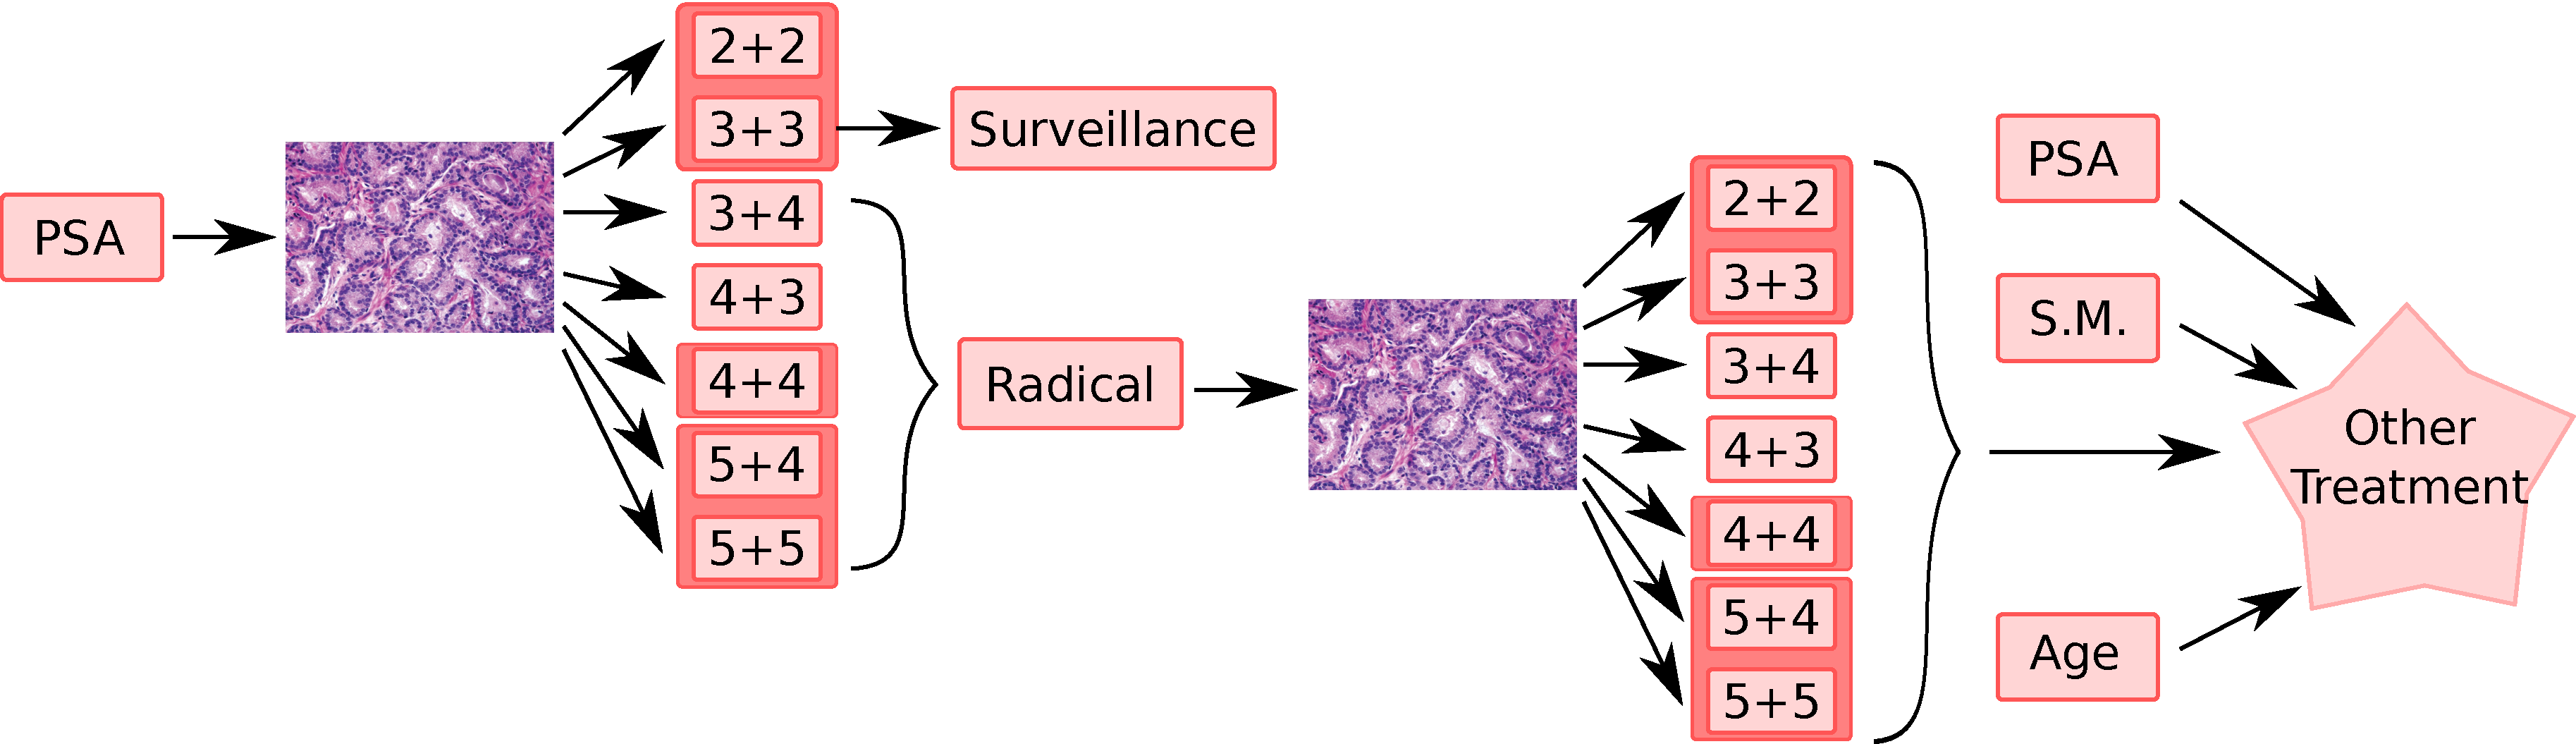
\includegraphics[width=\textwidth]{../figs/gleason/gleason-process}}

\end{frame}
%%%%%%%%%%%%%%%%%%%%%%%%%%%%%%%%%%%%%%%%%%%%%%%%%%%%%%%%%

%%%%%%%%%%%%%%%%%%%%%%%%%%%%%%%%%%%%%%%%%%%%%%%%%%%%%%%%%
\begin{frame}
\frametitle{Gleason Grading}
\framesubtitle{~}

    \begin{columns}
        \column{.45\textwidth}
        \centering
        \only<1>{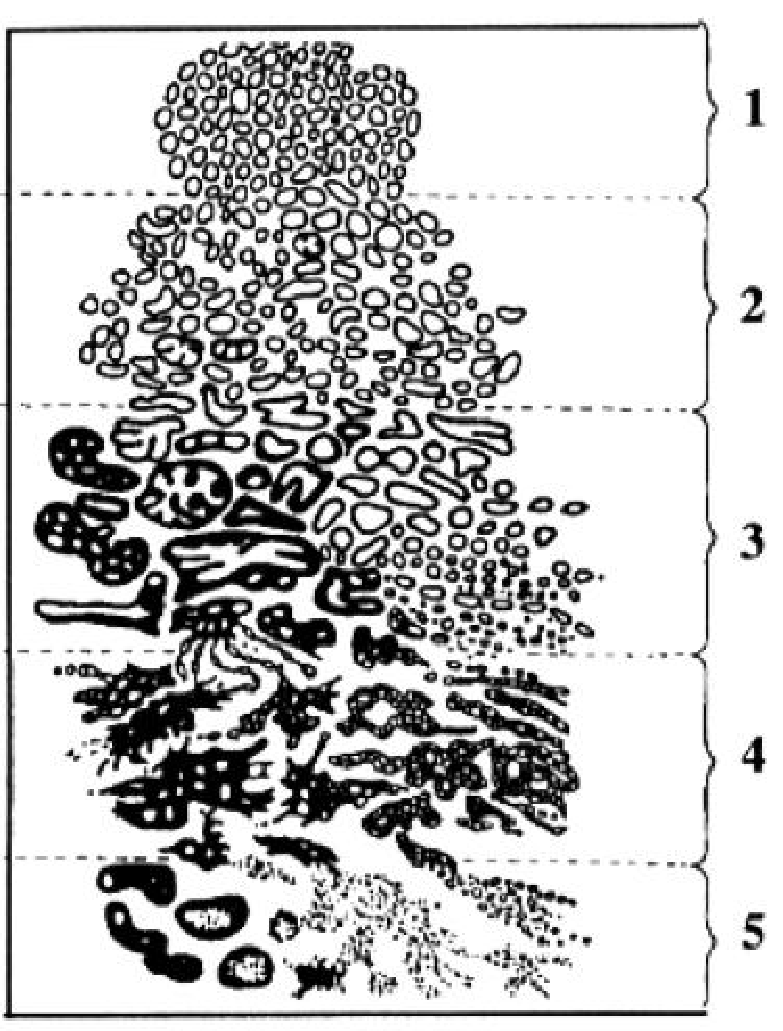
\includegraphics[height=2in]{../figs/gleason/gleason-old}}
        \only<2->{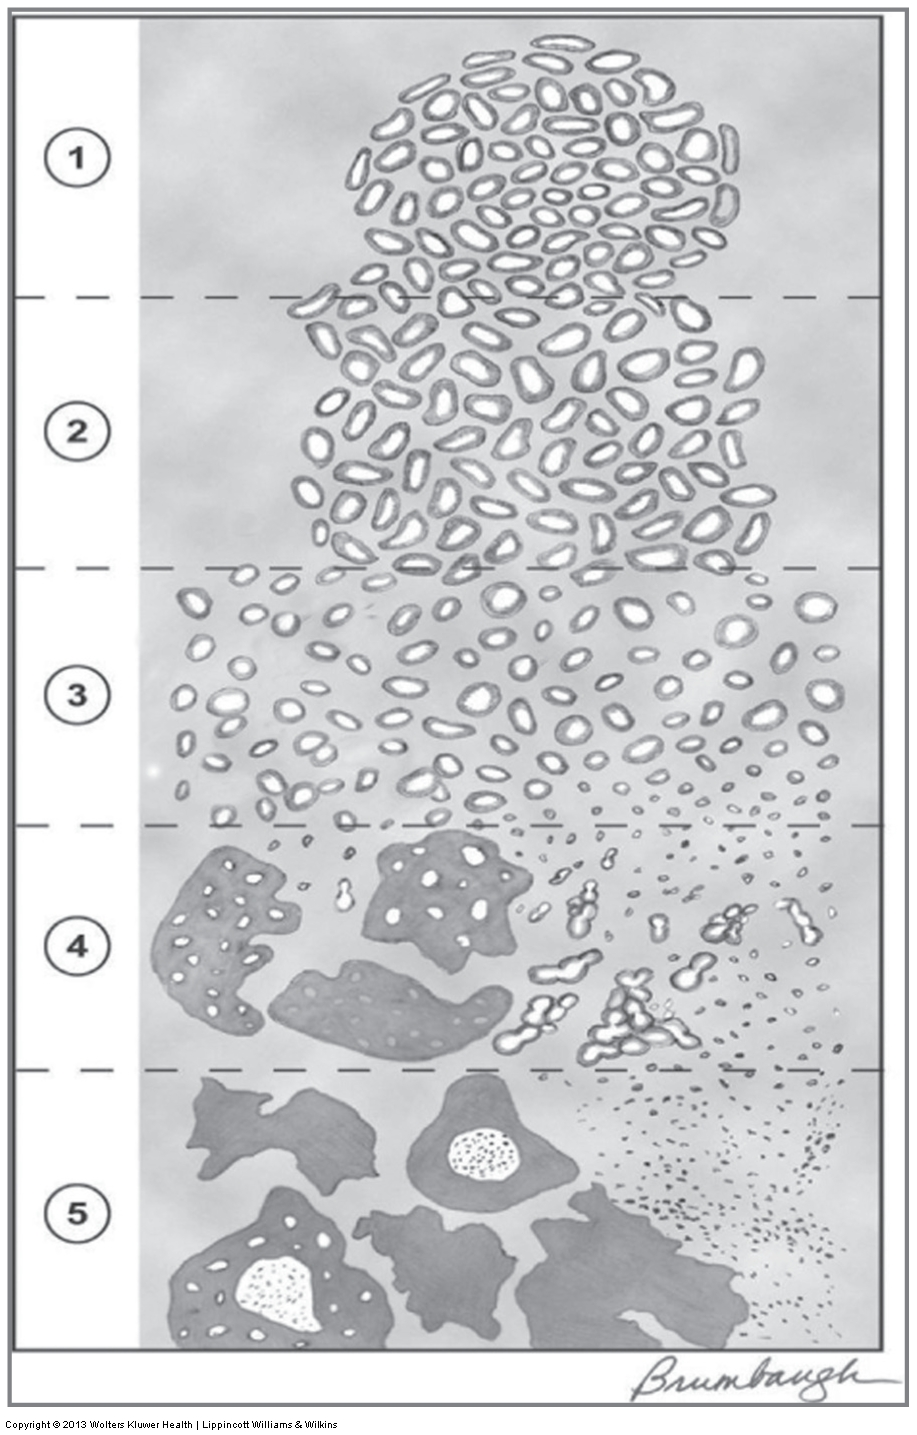
\includegraphics[height=2in]{../figs/gleason/gleason-new}}
        \column{.45\textwidth}
        \begin{block}{}
            \hangindent=1.5cm
            \hangafter=1
            \noindent
            Grade 1: well-defined, nicely packed

            \hangindent=1.5cm
            \hangafter=1
            \noindent
            Grade 2: larger, more tissue,  less uniform


            \hangindent=1.5cm
            \hangafter=1
            \noindent
            Grade 3: less defined glands%
            \only<1>{, some cribriform}

            \hangindent=1.5cm
            \hangafter=1
            \noindent
            Grade 4: fused glands, open lumens%
            \only<2->{, cribriform}

            \hangindent=1.5cm
            \hangafter=1
            \noindent
            Grade 5: no glandular definition, sheets of cells
        \end{block}
    \end{columns}
    \only<1>{\footnotetext{
        Donald Gleason, 1966, image from \emph{The Gleason Grading System: A Complete
        Guide for Pathologist and Clinicians} by Eppstein}}
    \only<2>{\footnotetext{
        2005 Consensus, image from \emph{The Gleason Grading System: A Complete
        Guide for Pathologist and Clinicians} by Eppstein}}

\end{frame}
%%%%%%%%%%%%%%%%%%%%%%%%%%%%%%%%%%%%%%%%%%%%%%%%%%%%%%%%%

%%%%%%%%%%%%%%%%%%%%%%%%%%%%%%%%%%%%%%%%%%%%%%%%%%%%%%%%%
\begin{frame}
\frametitle{Prostate Cancer}
\framesubtitle{Diagnosis}

\centering
    \onslide<1->{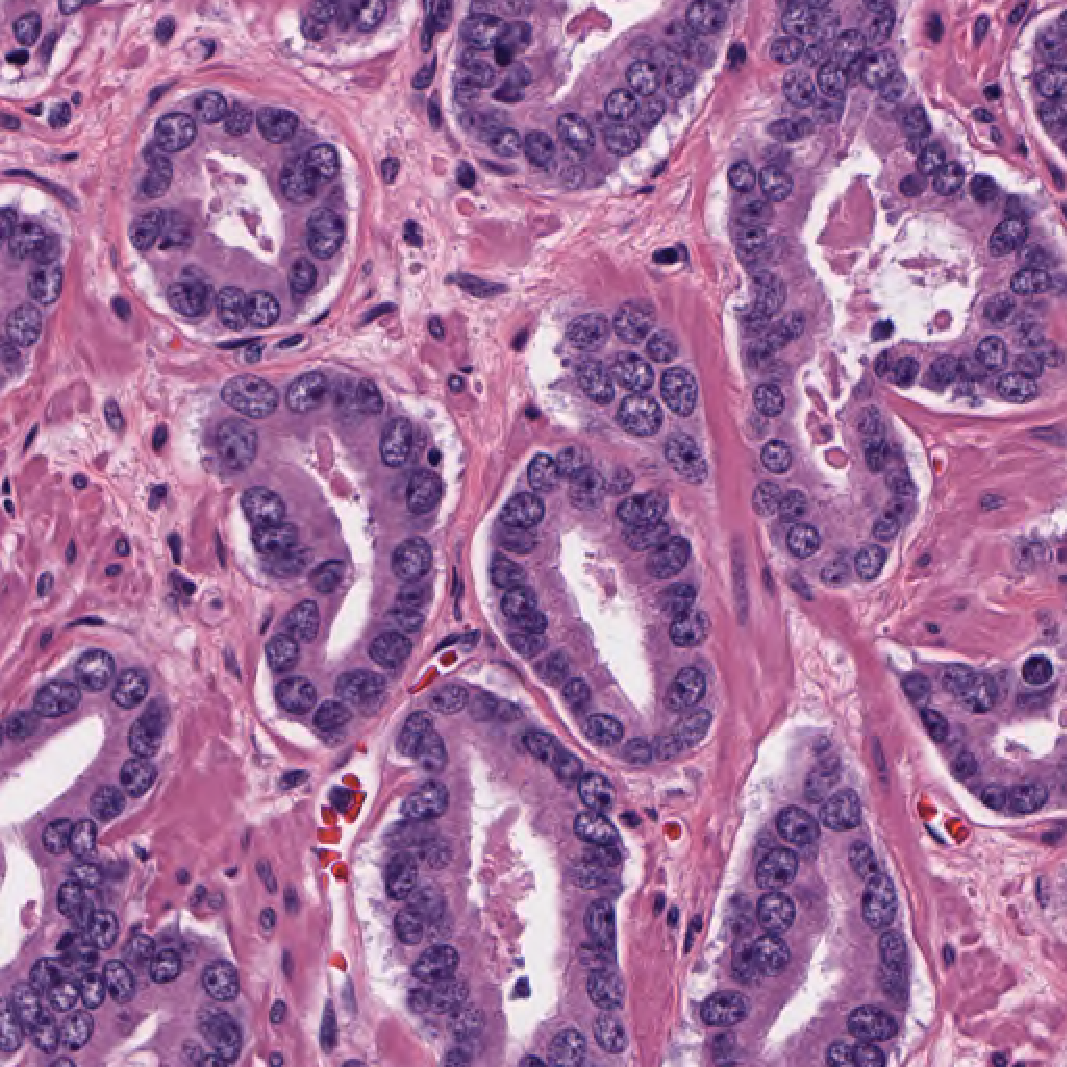
\includegraphics[width=.45\textwidth]{../figs/gleason/gleason3}}
    \quad
    \onslide<2->{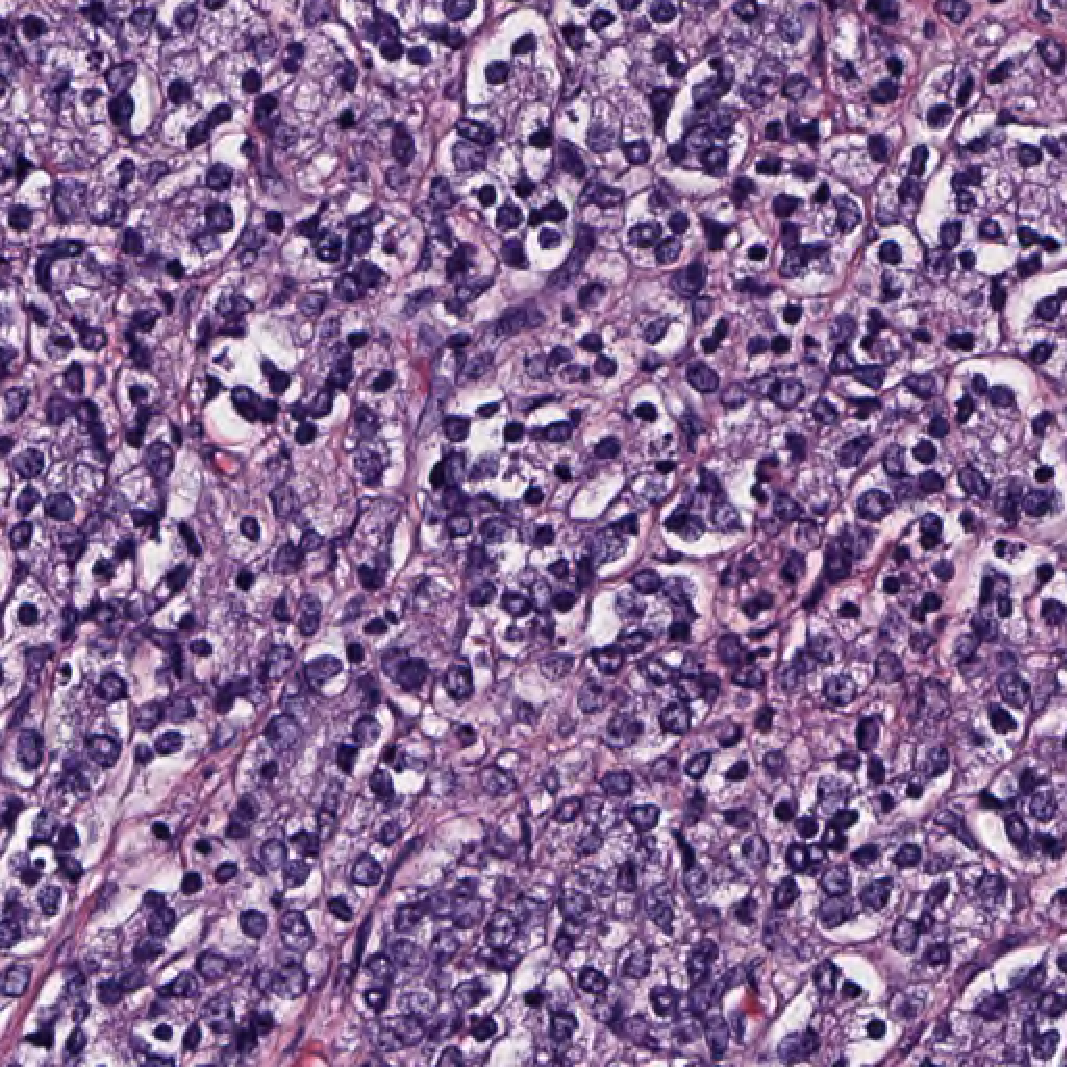
\includegraphics[width=.45\textwidth]{../figs/gleason/gleason5}}
\end{frame}
%%%%%%%%%%%%%%%%%%%%%%%%%%%%%%%%%%%%%%%%%%%%%%%%%%%%%%%%%

\frame<1->[label=compareGlands]{
\frametitle{}

\begin{block}{}
\centering
 \only<1>{
\includegraphics[width=.7\textwidth]{gleason/compare-0}}%
 \only<2>{
\includegraphics[width=.7\textwidth]{topology/inference-compare-1}}%
 \only<3->{
\includegraphics[width=.7\textwidth]{topology/inference-compare-2}}%
\end{block}

}

\begin{frame}
    \frametitle{Real Data}
    \framesubtitle{P.\ Lawson, J.Q.\ Brown, BTF, C.\ Wenk, A.\ Scholl, Sci
    Reports 9, 2019.}

    \begin{block}{}
        \centering
        \only<1>{
\includegraphics[height=2in]{gleason/tsne_fig_hist}}
    \end{block}
\end{frame}
